% This chapter should describe what was actually produced: the programs which
% were written, the hardware which was built or the theory which was developed.
% Any design strategies that looked ahead to the testing stage might profitably
% be referred to (the professional approach again).

% Descriptions of programs may include fragments of high-level code but large
% chunks of code are usually best left to appendices or omitted altogether.
% Analogous advice applies to circuit diagrams.

% Draw attention to the parts of the work which are not your own. Making
% effective use of powerful tools and pre-existing code is often laudable, and
% will count to your credit if properly reported.

% It should not be necessary to give a day-by-day account of the progress of the
% work but major milestones may sometimes be highlighted with advantage.

\chapter{Implementation}

\begin{center}
  \vspace*{5mm}
  \begin{tikzpicture}[node distance = 2cm, auto]
    % Place nodes
    \node [block_spaced] (input) {input};
    \node [block_spaced, right=of input] (processing) {data processing};
    \node [block_spaced, above=of processing] (storage) {data storage};
    \node [block_spaced, right=of processing] (output) {output formatting};
    \node [block_spaced, below=of processing] (command) {application logic};
    % Draw edges
    % \path [line] (input) -- (processing);
    \path [line, dashed] (processing) -- (storage);
    \path [line, dashed] (storage) -| (output);
    \path [line] (command) -- (input);
    \path [line] (command) -- (processing);
    \path [line] (command) -- (output);
  \end{tikzpicture}
  \\
  \emph{The structure of my project, as decided in Chapter 2}
\end{center}

\section{The Parser}
To implement my parser, I made use of an existing domain-specific language
available as a Ruby library called Treetop\cite{website:treetop}; Treetop allows
for easy implementation of Parsing Expression Grammars, which, simply put, are
grammars that built up out of a combination of rules and regular expressions.

Parsing Expression Grammars\cite{website:peg} were particularly appealing to me
for two reasons: firstly, they are essentially a more powerful version of
regular expressions, with which I am already familiar and secondly, they can be
made to run in constant time if implemented as a packrat parser, which Treetop
does. This constant time guarantee is provided by the process of memoization,
which trades off time for space by caching previous inputs and the resulting
parse trees to remove the need for repeated computations.

Treetop grammars are written as their own .treetop files, which are then used by
the \lstinline|tt| program to generate executable parsers. The end result is a
Ruby source file which can be included and used to parse the language defined by
the grammar. Treetop also allows you to define a class that nodes within the
parsed data should be instantiated as, this means that nodes can be given
methods with which they can parse themselves or their children; which is much
preferable to the traditional methods of writing code to walk the tree
structures.

\begin{code}[language=treetop]
  rule comment
    '//' ( !EOL .)* EOL <CommentNode>
    / '# ' ( !EOL .)* EOL <CommentNode>
    / (multiline_comment) <CommentNode>
  end
  rule multiline_comment
    '/*'
    (
      !'*/'
      (. / EOL)
    )*
    '*/'
  end
  rule EOL
    [\n]
  end
\end{code}

Above is a snippet from my Treetop grammar for C, defining the grammar for
comments. The rule \lstinline|comment| contains an ordered choice of expressions
that define each type of comment available in C, and informs Treetop that they
should be instantiated using the class \lstinline|CommentNode|;
\lstinline|CommentNode| defines a method with which the text of the comment
can be extracted.

The parser takes the contents of a file and, provided that they are `valid' C
(as understood by my parser), produces a parse tree which instantiates the
classes I defined for the appropriate nodes. This tree can then be navigated
using the methods I implemented in the classes.

  \subsection{Regression Testing}
    To ensure that I was properly implementing my grammar for C, I wrote some
    tests for my parser that would check that parsing a particular piece of code
    would yield a valid result. This was the quickest and easiest way of
    building up a working grammar for the language and allowed me to be
    confident that what I had written would function correctly as I moved
    forward.

    This was implemented using \lstinline|TestCase|, a class that is part of the
    Ruby standard library, and simply involves defining methods that execute the
    code required for each test and uses various types of assertions to ensure
    that the results are as expected.

    The process went as follows:

    \begin{center}
    \begin{tikzpicture}[node distance = 2cm, auto]
        % Place nodes
        \node [block] (init) {write tests for new syntax};
        \node [block, below=of init] (run) {run the tests};
        \node [decision, below=of run] (fail) {does it fail?};
        \node [block, left=of fail] (debug) {another rule in the grammar is
          parsing incorrectly};
        \node [block, below=of fail, node distance=3cm] (develop) {add new rules
          to the grammar};
        \node [block, below=of develop, node distance=3cm] (rerun) {re-run the
          test};
        \node [decision, right=of rerun] (refail) {does it fail?};
        % Draw edges
        \path [line] (init) -- (run);
        \path [line] (run) -- (fail);
        \path [line] (fail) -- node[decision answer] {no} (debug);
        \path [line] (fail) -- node[decision answer] {yes} (develop);
        \path [line] (develop) -- (rerun);
        \path [line] (rerun) -- (refail);
        \path [line] (refail.east) |- node[decision answer] {no} (init);
        \path [line] (refail) |- node[decision answer] {yes} (develop);
    \end{tikzpicture}
    \end{center}

  \subsection{Parsing Problems}
    As I wrote my initial grammar for the C parser, it became apparent that I
    was having some problems; I got to the point where implementing new rules
    would cause other tests to fail, the problem was that describing C correctly
    required such a large enough grammar that the rules were interacting in ways
    I had not accounted for. This meant that progress on the grammar slowed to a
    crawl, and it became apparent that the grammar would need to be largely
    rethought to fully parse C.

    Whilst having a grammar that understood all of the C language would be
    ideal, such a parser would be slower than necessary and capture more detail
    than was required, therefore I wrote a new, simpler parser that understood
    how to navigate through the C files and parse at the top level, rather than
    parsing all of it.

    Instead of parsing function bodies, the simplified parser contains rules to
    match pairs of braces within functions, ignoring those in strings and
    comments, to understand where functions begin and end. With global variable
    assignments, the parser has rules to match from an equals sign to the
    semicolon at the end of the line. These simplifications allowed for me to
    dispense with the expensive and complicated parsing of control structures
    and arithmetic, and reduced the grammar from ${\sim}$500 lines in the
    original (unfinished) grammar to ${\sim}$300 lines for the completed
    simplified one.

    Ideally, some or all of the more complex behaviour would be restored to the
    grammar, as it would allow for better analysis of the parsed language, such
    as including in the documentation what was referenced by a particular
    function. Given the time constraints involved in the project, this could not
    be performed.

\section{Handling the Data}
After the source files have been parsed into a parse tree, the useful data can
be extracted; using the methods that were added into the parse tree by Treetop,
the code runs through the functions, variables and other pieces of data and
pulls out the needed information to be stored in the database.

To store the data I opted to use SQLite, as it requires no configuration to use
and stores all data in a file, rather than on a SQL server; this means that no
setup of databases is required on the part of the user. I used the
sqlite3\cite{website:sqlite} Ruby library to interact with my database, which
allows you to interact with data from the database using the normal Ruby types.

\begin{center}
  \vspace*{5mm}
  \begin{tikzpicture}[node distance = 2cm, auto]
    % Place nodes
    \node [block_spaced] (processing) {initial processing};
    \node [block_spaced, above=of processing] (storage) {data storage};
    \node [block_spaced, right=of processing] (post) {post processing};
    % Draw edges
    % \path [line] (input) -- (processing);
    \path [line, dashed] (processing) -- (storage);
    \path [line, dashed] (storage) -| (post);
    \path [line, dotted] (post) |- (storage);
    \path [line] (processing) -- (post);
  \end{tikzpicture}
\end{center}

This section actually breaks down into the the above layout; processing must be
performed in two stages, this is because some of it cannot take place until
after all the files have been parsed.

  \subsection{Processing}
    The classes I defined for use in the parse tree provide easy access to the
    data within the nodes, and their subtrees, whilst masking the specifics of
    the tree itself; this means that future additions to the parser and the way
    in which it works will not affect the processing of the data. In addition,
    this allows for the reuse of the processing code on the parse trees of
    different languages, provided that the nodes in that tree expose the same
    methods.

    When extracting the data from the parse tree, I ended up with two hashes
    describing a function: one using the details from the function definition
    itself, and the other from the documentation string associated with it.
    Since some functions in the source being parsed may only be partially
    documented, I needed to account for this in my code to ensure that the
    resulting data was consistent; in particular, if a function is documented
    the hash containing information about the prototype will contain extra
    information. Uniting the arguments with their documentation proved
    interesting, and I had to attempt to write code to manage it several times
    before I created a solution that provided an appropriate output regardless
    of input.

    \begin{code}[language=ruby, gobble=6]
      if function.documented?
        prototype[:arguments] = prototype[:arguments].zip(prototype[:params]).map do |a,d|
          d ? a.merge(d) : a
        end
        prototype.delete(:params)
      end
    \end{code}

    This small section of code was the eventual solution, and in just a few
    lines accomplishes quite a bit. The array containing the arguments
    parsed, from the function prototype itself, is merged with the array
    containing the documentation for each argument, producing a new array. This
    array is contains several arrays, each holding the documentation and
    prototype for one argument; finally, the map function returns the array I
    need by merging the two hashes together, if the argument is documented, or
    returning the just the argument's hash if no documentation exists. The
    example data below demonstrates the process.

    \begin{code}[language=ruby, gobble=6]
      A = [{a => 1}, {b => 2}, {c => 3}]
      B = [{d => 4}, {}, {f => 6}]

      # After zipping A & B...

      C = [[{a => 1}, {d => 4}], [{b => 2}], [{c => 3}, {f => 6}]]

      # After mapping C...

      D = [{a => 1, d => 4}, {b => 2}, {c => 3, f => 6}]
    \end{code}

    The arrays A \& B represent the arguments from the function definitions
    and the arguments from the documentation string, respectively; D
    represents the combined information returned, C is an intermediate step,
    shown here for clarity.

      \subsubsection{Post-processing}
        Once the data for all files in the directory has been added to the
        database, some extra processing takes place to resolve which files
        include one another. By looping through all the includes encountered
        and determining whether it refers to another file that has been
        processed, links are built between files, which are later used by the
        output stage to allow a user to jump from one file to one of its
        includes easily.

        To determine if one file refers to another, I decided to check whether a
        following the path described in the include results an a file that
        exists, relative to that file. This is by no means a fool-proof
        solution, as it does not take into account the include paths passed to a
        compiler, but the only other sensible solution to this problem would be
        to also parse the Makefile (or similar file in another build system) to
        extract the include paths used. Given the number of different build
        systems used and the time taken to implement another grammar for parsing
        any of them, I concluded that this was not a valid solution in the time
        available.

  \subsection{Storage}

    The sqlite3 Ruby library made interacting with my database very natural, SQL
    statements are executed with a method that takes a query string and results
    are returned as a \lstinline|ResultSet|, which can be enumerated just like
    an array. Additionally, each result can either be represented as an array or
    a hash; I found using hashes much more natural because it allows you
    explicitly refer to columns, like so:

    \begin{code}[language=ruby, gobble=6]
      db = SQLite3::Database.new("db.sqlite")
      db.execute("SELECT * FROM files").each do |result|
        puts "The file with #{result['id']} has path: #{result['path']}"
      end
    \end{code}

    Since everything parsed by my software originally comes from one of a set
    of files, it was natural that my database revolved around the same
    concept; as such, all the information stored in my database is linked back
    to the file it came from. The diagram below shows the layout of my
    database, with the arrows representing the links between tables with foreign
    keys; all bar two of the tables reference the ID of the file they are
    contained in, `arguments' and `elements' refer to the ID of the structure
    they were contained in, which in turn refers to the file.

    \noindent\makebox[\textwidth]{%
      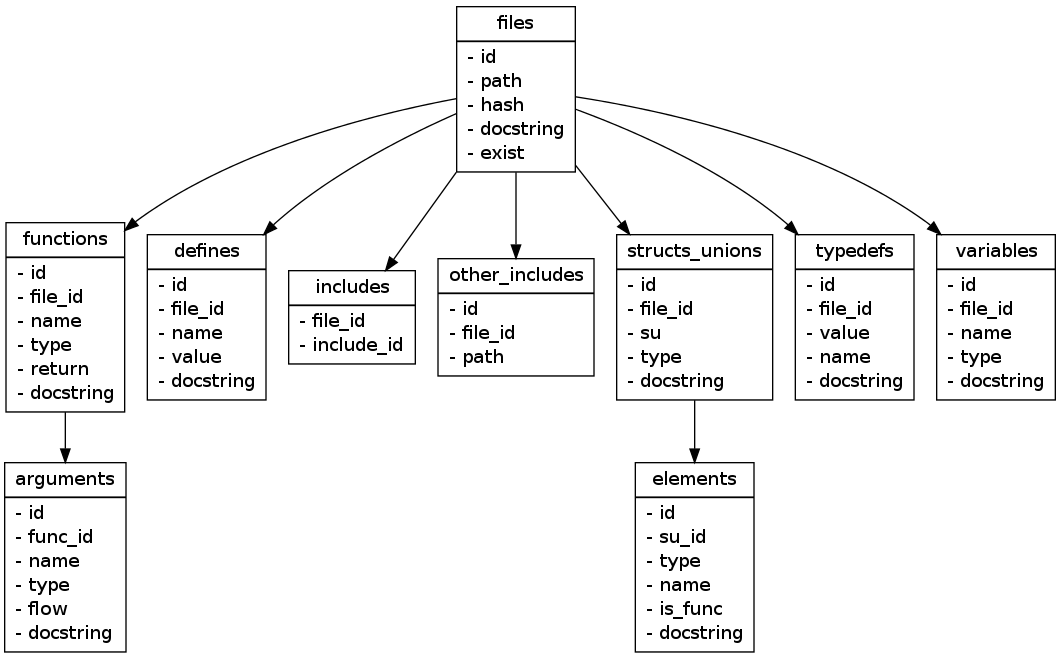
\includegraphics[width=160mm]{db.png}
    }

    Having foreign keys running through my database like this ensures that
    nothing can be inserted with a non-existent ID, thereby reducing insertion
    anomalies, but it also gained me a second advantage: when defining foreign
    keys in SQL, it is possible to design what happens when a particular entry
    is deleted. I specified in my table creation statements that when the
    entry a particular key references is deleted, the entry referencing it is
    also deleted; since every table in my database has a foreign key, a
    deletion of a file in the `files' table cascades all the way through,
    removing all the data about that file. This ensures that there is never
    any stale data kept in the database, which will improve run time by
    keeping the data sets smaller.

    This is preferable to deleting anything manually, as it removes the
    chances for error; it also eliminates the time it would take to query each
    table in the database and work out what to remove.

    The files are stored in the database by their path, relative to where the
    software is executed; this means that two files with the same name cannot
    interfere with one another, since they are distinct as far as their paths
    are concerned.

    When a source file is updated, and the software re-run, the hash of the file
    no longer matches the one stored in the database; at this point the entry
    from the files table is deleted, thereby removing all the other data
    relating to that file from the database due to the cascading deletion. The
    details of the new version of this file are then inserted into the database
    as before. This approach is much simpler than the alternative, which would
    involve updating some entries, inserting others and removing out-dated
    information. In addition to being more complicated, this method would also
    be more error-prone; since leaving behind stale information, such as an
    entry in the arguments table, could lead to the function being displayed
    in the output as having extra arguments.

    The structure of my database made it easy to define powerful queries in
    SQL, that gave me the data I needed more easily than if I'd extracted all
    the data separately and combined it in Ruby. Database engines are also
    optimised for this type of data manipulation. I could have made my data
    retrieval faster by creating indices on some of the columns that were
    commonly queried against in the database; however the number of insertions
    into the database is much higher than the queries against the data, so I
    felt that the end result have been likely to have been slower due to the
    insertion overhead with indices.

    \begin{code}[language=sql, gobble=6]
      SELECT types.*, files.path FROM
       (SELECT id, file_id, name, 'typedef' FROM typedefs WHERE typedefs.name = ?
        UNION ALL
        SELECT id, file_id, name, 'define' FROM defines WHERE defines.name = ?
       ) AS 'types' INNER JOIN files ON types.file_id = files.id
    \end{code}

    This SQL statement looks up a type in the \lstinline|typedef| and
    \lstinline|define| tables, unioning the two result sets together to ensure
    that we get results from either, and then performs an inner join of these
    results against the files table to get the information on the file that the
    typedef or define was found in. This results in a rather large SQL
    statement, which can be a little complicated to understand, however it is
    much quicker than running three queries and producing the result in Ruby.

\section{Generating the Output}

Once all the data has been processed and stored, the output can be generated;
currently there is only one available output format, HTML, however the
outputting process has been designed so that a new output format can be easily
added. To do this, a generic \lstinline|Output| class was created that defines
methods that can be used to extract all the data required for producing the
output, these methods provide easy access to all the queries commonly needed to
produce documentation. This means that creation of a new output format only
requires the definition of a new subclass of \lstinline|Output| that defines an
\lstinline|output| method, which can call the other methods already defined to
get its data.

Initially, I considered generating XML from the required elements in the
database, and then using XSLT to create the final documents, but the XSLT
processor libraries available for Ruby did not provide enough documentation for
me to feel comfortable using them in this instance.

The \lstinline|HTMLOutput| class creates an overview page, listing all the files
that were parsed and an excerpt of their file-level documentation (if any
exists), and then extracts the data for each file from the database and creates
an HTML file for each. These files are placed within directories that match the
structure of the original codebase, allowing for convenient navigation by the
user to the correct location and making it easier to link between files.

Generating output can be a messy process, especially with HTML, as inevitably
code and HTML markup end up being interleaved together; I have done my best to
separate the two out by defining functions that produce particular sections of
commonly repeated HTML, such as creating links and table rows, to increase the
readability of the code, however there is only so much this can be done.

\begin{code}[language=ruby, gobble=2]
  def row_with_id(id, *entries)
    if entries == []
      "<tr id=\"#{id}\"></tr>"
    else
      "<tr id=\"#{id}\"><td>#{entries.join("</td><td>")}</td></tr>\n"
    end
  end
\end{code}

The function above allows me to create a new row in a table
\lstinline|row_with_id("some_id", ["item1", "item2"])| when I need one, rather
than repeating the same HTML over and over. String interpolation also helps the
situation greatly, as it allowed me to write much more concise code; the above
code without it would have been much more verbose and complicated.

This would have also been more expensive to compute, as it requires mutating the
string four times, rather than just creating it correctly in the first place.
This is one example of a reason I chose Ruby in my proposal.

While generating the output the code checks if `style.css' already exists in the
output directory, if there is not one already present, a default one is created.
This file is referred to in the HTML files, and contains all the relevant CSS
markup needed by the browser to layout the documentation in a sensible manner.
This can be modified or replaced by the user to suit their needs; all important
HTML elements in the output files have IDs or classes associated with them,
allowing for convenient styling of the documents.

\noindent\makebox[\textwidth]{%
      \includegraphics[width=160mm]{output.png}
}

  \subsection{Linking Between Files}
    Linking between the output pages, for things like the list of includes, was
    solved using \lstinline|Pathname|, another class available in the Ruby
    standard library. \lstinline|Pathname| allows you to determine the relative
    path between two files; since I had ensured that the directory structure of
    my outputted data matched that of the input data, the relative path between
    the two source files is also the relative path between the HTML files. This
    meant that producing these paths was fairly easy.

    Taking this a step further, I also implemented linking a type to the file it
    was originally declared in; this was done with \lstinline|Pathname| as
    above, and a \lstinline|type| method in \lstinline|Output| that looks up
    types in the SQLite database.

    Since all the files generated use exclusively relative paths to other files,
    the output directory can be relocated to anywhere else and the files will
    still correctly refer to one another. This is important, since documentation
    will often be moved to other locations, such as a webserver, for later
    viewing.

\section{Application Logic}

The application logic coordinates the stages of program and ensures that the
correct options are passed to them, it is also where the traversal of
directories to find the files to be parsed takes place; Ruby's use of blocks
allows the code for this to be written quickly and clearly. I wrote a small
method, \lstinline|recurse|, that recurses down through the directories
contained within a particular path, and yields the files contained in them back
to its caller. This way of doing this made working through the files as
convenient as working through the elements of an array, without having to store
all of the filenames in an array first.

The application logic handles building documentation incrementally; this is done
by calculating the MD5 checksum of each file before it is parsed, if it matches
the existing entry for that file in the database then the file is unchanged
since last time the program was run. This allows for the program to run much
quicker, and not have to do any redundant parsing.

Finally, it also handles removing old entries from the database; when the
program starts all files are marked as not existing, by setting the value of
`exist' in the files table of the database to 0, then as each file is
encountered its entry is updated to reflect that. After running over all the
files, any that still have their `exist' value still set to 0 are determined to
have been removed, and so their information in the database is deleted.

The whole process goes as follows:

\begin{center}
    \begin{tikzpicture}[node distance = 0.5cm, auto]
        % Place nodes
        \node [block] (exist) {mark all database entries as exist=0};
        \node [block, left=of exist] (check) {check extension};
        \node [decision, below=of check] (extension) {correct?};
        \node [decision, left=of extension] (next) {next file};
        \node [block, below=of extension] (md5) {generate MD5 of file};
        \node [decision, below=of md5] (match) {hash match?};
        \node [block, below=of next] (mark) {mark file as exist=1};
        \node [block, below=of match] (parse) {parse the file};
        \node [decision, below=of parse] (success) {success?};
        \node [block, below=of success] (process) {process the parse tree};
        \node [block, left=of next] (delete) {delete database entries where
          exist=0};
        % Draw edges
        \path [line] (exist) -- (check);
        \path [line] (check) -- (extension);
        \path [line] (extension) -- node[decision answer] {yes} (md5);
        \path [line] (extension) -- node[decision answer] {no} (next);
        \path [line] (md5) -- (match);
        \path [line] (match) -| node[decision answer] {yes} (mark);
        \path [line] (match) -- node[decision answer] {no} (parse);
        \path [line] (parse) -- (success);
        \path [line] (success) -| node[decision answer] {no} (mark);
        \path [line] (success) -- node[decision answer] {yes} (process);
        \path [line] (mark) -- (next);
        \path [line] (process) -| (mark);
        \path [line] (next) |- node[decision answer] {yes} (check);
        \path [line] (next) -- node[decision answer] {no} (delete);
    \end{tikzpicture}
\end{center}

\section{The Command-Line Interface}
The command line interface ties all of the previous stages together, allowing
for everything to be used together conveniently without requiring any Ruby
knowledge on the part of the user.

Aside from making the process more convenient, the command line interface also
provides easy manipulation of the options the program uses and performs the
cleaning and the initial setup of the database.

  \subsection{Option Parsing}
    Ruby has an extremely robust command-line option parser built into the
    standard library, so there was no need to roll my own or make use of an
    external library. \lstinline|OptionParser| made defining options simple, and
    produces help text automatically, so the whole process was quite straight
    forward.

    The following snippet is sufficient to describe a verbose option for a
    program:

    \begin{lstlisting}[language=ruby,gobble=6]
      options = {}
      OptionParser.new do |opts|
        opts.banner = "Usage: example.rb [options]"

        opts.on("-v", "--[no-]verbose", "Run verbosely") do |v|
          options[:verbose] = v
        end
      end.parse!
    \end{lstlisting}

    Using \lstinline|OptionParser| allowed me to specify default options within
    my \lstinline|options| hash, which can then be overridden by the user on the
    command-line.

    \lstinline|OptionParser| also allows you to define an option that takes only
    certain inputs, using this it was easy to create and option for choosing the
    output format; even though there is only one currently, this project was
    designed with extensibility in mind.

    \begin{code}[language=ruby, gobble=6]
      o.on("--format FORMAT", outputs, "Select output format",
           "  (#{outputs.keys.join(", ")})") do |format|
        options[:format] = format
      end
    \end{code}

    This adds an option that will accept any entry that is a key in the
    \lstinline|outputs| hash, and sets the appropriate entry in the
    \lstinline|options| hash to the value of the entry, which is the output
    class to use. This means that adding a new output format requires only a
    subclass of \lstinline|Output| and an entry referencing it in the
    \lstinline|outputs| hash.
